% 原书第 1 页（PDF 第 14 页）
\BookPage{1}{14}
\BookHeading{长松献寿繁花颂}{长松献寿繁花颂}{王耀庭*}
\BookSubheading{（壹）}

台北国立故宫博物院藏有清陆㬙（意同𬀩）〈长松图〉及乾隆时期〈缂丝大寿字〉。先说清陆㬙〈长松图〉。（图1）

纸本。纵三一五‧九公分；横一二九‧一公分。

着色画。款：「云间陆㬙」。钤印一：「㬙」。

收传印记：乾隆御览之宝。石渠宝笈。养心殿鉴藏宝。嘉庆御览之宝。宣统御览之宝。著录于《石渠宝笈》初编、《故宫书画图录》。\BookRef{1}

关于陆㬙生平，见张庚《清朝画征录》：

\begin{BookQuote}
陆痴名㬙，字日为。华亭人。性狷癖。故人以痴呼之。善山水，自成一局。其法用挑笔密点，由淡及浓，不惜百遍。林峦崖石间，烟云纠缦，墨气𬘡缊，亦可喜也。其布置务求奇僻，不肯作常蹊，能为寻丈大幅。浙江巡抚屠公，馆之西湖，逾年而卒。屠公为之归其葬。\BookRef{2}
\end{BookQuote}

陆㬙作品出现于康熙朝，然「浙江巡抚屠公」一句不正确，有清一朝，无屠姓居浙江巡抚。又案《桐阴论画》载，与《清朝画征录》相同之外，别有评语：

\begin{BookQuote}
余见册页画幅，干笔皴擦，用淡墨笼染，一种奇古之气，与程穆倩相伯仲，境界灵异，别有会心，非巧思力索所能造也。\BookRef{3}
\end{BookQuote}

\vfill
\begin{BookNotes}
\BookNote{*}{国立故宫博物院退休。}
\BookNote{1.}{国立故宫博物院编《秘殿珠林石渠宝笈》初编。（台北：故宫，1971），页675。国立故宫博物院编《故宫书画图录》（十一）（台北：故宫，1991。），页133。}
\BookNote{2.}{清张庚《清朝画征录》（台北：新兴，1956），卷中，页12。}
\BookNote{3.}{清秦祖永《桐阴论画》三编，上卷，页2。。收入《续修四库全书》子部艺术类，（上海：上海古籍，1955），1085册。总页373。}
\end{BookNotes}

% 原书第 2 页（PDF 第 15 页）
\BookPage{2}{15}
\par\addvspace{4pt}\noindent
\begin{minipage}[t]{0.526\linewidth}
\vspace{0pt}
\noindent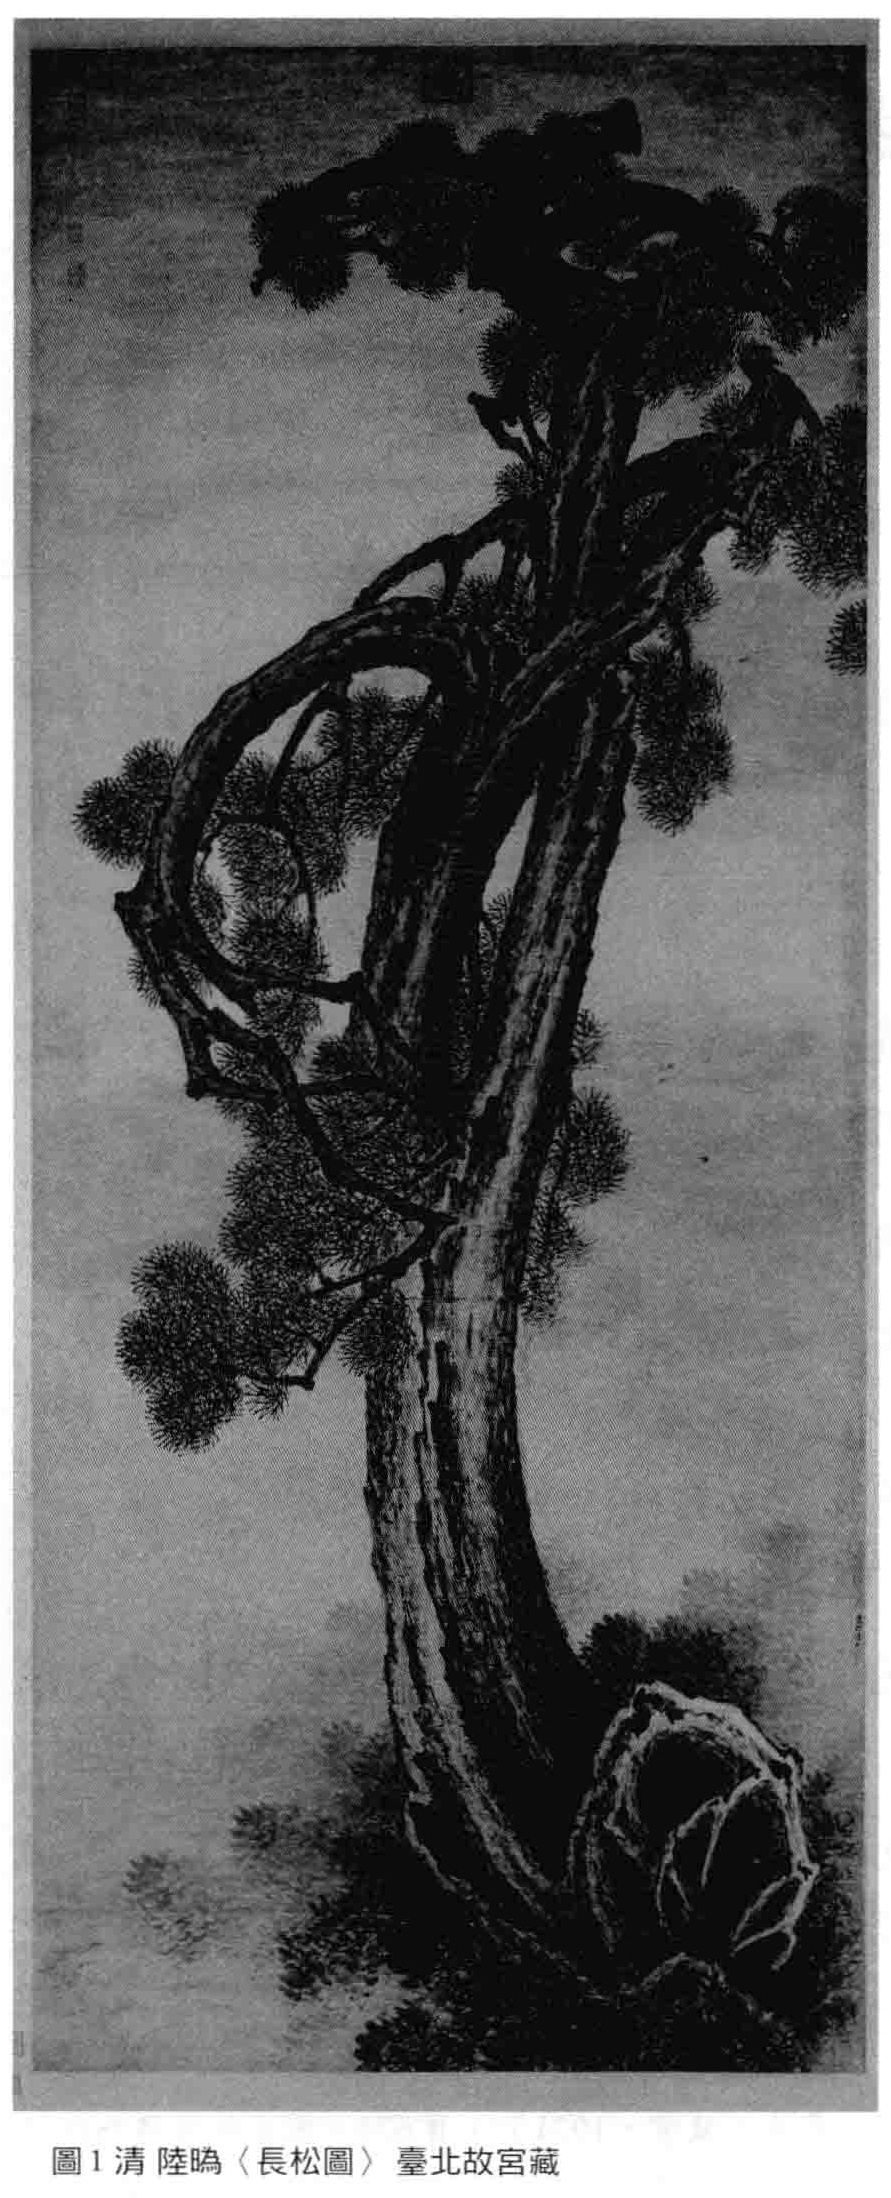
\includegraphics[width=\linewidth,height=.81\textheight,keepaspectratio]{assets/p015-01.jpg}
\end{minipage}
\hfill%
\begin{minipage}[t]{0.449\linewidth}
\vspace{0pt}\setlength{\parindent}{1.5em}
又曾于美国西雅图一私人收藏，见陆㬙《山水册》，后有引《娄县志》之跋文，较富传奇性之记载：

陆㬙浙江人。..画宗二米（米芾，1051-1107。米友仁，1074-1151）、房山（高克恭，1248-1310）。后参以己意，自成一家。所居在超果寺南，欲得其画者，每入寺，登一览楼，望其家炊烟，至午后不起，乃持银米易之，否则终不可得。故人以痴目之。(图2)

本幅纵高超过三公尺，是一幅相当巨型的作品。符合「能为寻丈大幅」的记载。在这样大的尺幅中，只画长松一株，凌空而起，在画幅中段，一干分为两木，枝干偃俯，纠结盘错之间，气势雄伟坚壮。枝干用粗笔划出，雄健挺拔；松针则用细笔密实点染，在在都显得厚实有力，画出了松的苍劲。画松干用钝笔皴擦，画坡地松影，用淡墨笼染。

本幅画法最为特殊者是描绘出光影，整幅处处存在于笔下。幅上方的天空背景，以墨染出云影，越下越淡，且左右交错，至中幅又见浓云横于松干背

\end{minipage}
\par\addvspace{4pt}

后，至于幅下，则松影在地。松针的影，更分出前后几层，松干之下，阳光不到处近于黑，周边越远越淡，分明光影迭


% 原图说　图1　清陆㬙〈长松图〉　台北故宫藏

% 原书第 3 页（PDF 第 16 页）
\BookPage{3}{16}
\noindent 覆，犹如徘徊反映于水镜之中。松干以光之照临，受阳光者虽有着笔，却是淡化，显得白光，光未到处，背者阴，以赭石浓墨染，如此作为，也就倍觉空间前后层次分明，松干立体圆浑。画法符合「林峦崖石间，烟云𫄙缦，墨气𬘡缊。」的传统陈述，其实这是大气与光线的传达。

相对于前人松干的画法，松的特征是鳞状的树皮，中国画中难免就「程式化」，以圆圈来表达，而无视实际的眼之所见。对树干的圆体状表现，从南宋刘松年画松，在树干中间留下一条纵贯不画的空白，不能说没有意会的受光所呈现的阴阳与立体感，却也是不脱「程式化」（图3）。本幅画松干，无一笔「圈鳞」，而是以短促直线，一笔一笔来描绘松干，松干「皴」皮的「密点由淡及浓，不惜百遍。」在这幅画上也得到验证。画松的质感掌握，体现了对自然的反应。整幅来看，确实是有别于从前到当时人的画法。

\BookArt{p016-01.jpg}{0.990}{0.370}

\noindent 上引画史，说陆㬙「后参以己意，自成一家。」这「参以己意」的「己意」从何而来？简短的陆㬙相关资料中并没有提出任何解说。活动于康熙时代的陆㬙，画上出现西洋的光影画风，并不足为奇。只是论明清之际，中国画受到西洋的影响，研究史上从未以陆㬙的画风作举证。简短回顾洋风在中国的发展，总以欧洲在十六世纪初


% 原图说　图2　陆㬙《山水册》　咸丰六年（1856）立泉跋文　美国西雅图私人藏
% 原图说　图3　传南宋刘松年〈斗茶图〉画松「程式化」　台北故宫藏

% 原书第 4 页（PDF 第 17 页）
\BookPage{4}{17}
\noindent 期，开始大肆向外扩张，东西双方由于商业的频繁接触以及宗教热忱所需，许多西方美术作品因而引进了中国。介绍西洋美术作品的媒介，首推天主教的耶稣会传教士，他们往往利用美术品作为传教的工具，明神宗万历二十八年（1600）来华的利玛窦(MateoRicci,1552-1610)，在上神宗的奏疏上说：

\begin{BookQuote}
谨以原携本国土物，所有天帝图像一幅、天帝母图像二幅、天帝经一本、珍珠镶嵌十字架一座、报时自鸣钟二架、万国图志一册、西琴一张，陈献御前。4
\end{BookQuote}

这份奏章，向被认为是西洋画传入中国最早的文献。姜绍书的《无声诗史》对此做解释：

\begin{BookQuote}
利马窦携来西域天主像，乃一女人抱一婴儿，眉目衣纹，如明镜涵影，踽踽欲动，其端严娟秀，中国画工无由措手。5
\end{BookQuote}

顾起元的《客座赘语》，记「利马窦」更详细：

\begin{BookQuote}
利马窦，西洋欧罗巴国人也…所画天主，乃一小儿；一妇人抱之，曰天母。画以铜版为帧，而涂五采于上，其貌如生。身与臂手，俨然隆起帧上，脸之凹凸处，正视与生人不殊。人间画何以致此？答曰：『中国画但画阳不画阴，故看之人面躯正平，无凹凸相。吾国画兼阴与阳写之，故面有高下，而手臂皆轮圆耳。凡人之面正迎阳，则皆明而白；若侧立则向明一边者白，其不向明一边者耳鼻口凹处，皆有暗相。吾国之写像者解此法以用之，故能使画像与生人亡异也。』
\end{BookQuote}

「吾国（西洋）画兼阴与阳写之」，而「中国画但画阳不画阴」，正其差异之处。画「阴」就是以相对的阴暗色彩，「凡人之面正迎阳，则皆明而白；若侧立则向明一边者白，其不向明一边者耳鼻口凹处，皆有暗相。」这种「暗相」是当时中国人所无法接受的。从存留的实际作品，如肖像画的脸部处理都是同一色调的浓淡为层次。即使如郎世宁这批来华的传教士画家，以油画为清宫帝后画像，乃至其他动物植物题材，也极少出现「暗相」。

\vfill
\begin{BookNotes}
\BookNote{4.}{《熙朝崇正集》，收录于《中外交通史丛刊》第19册（北京：中华，2006），卷二，页19。}
\BookNote{5.}{姜绍书《无声诗史》收入《画史丛书》二（台北：文史哲，1974)，卷七，西域画。页133。}
\BookNote{6.}{明顾起元《客座赘语》。收入《丛书集成新编》八八。（台北：新文丰，1985），卷六，页18-19。总页479。}
\end{BookNotes}

% 原书第 5 页（PDF 第 18 页）
\BookPage{5}{18}
面对洋风，当时知名的画家作出评论反应的，惟见吴历（1632-1718）与邹一桂（1686-1766）。吴历是天主教神父，邹一桂任职清朝高官，看过西洋美术品，应无疑义。邹一桂着《小山画谱》，有「西洋画」一条：

\begin{BookQuote}
西洋善勾股法，故其绘画于阴阳远近，不差锱黍。所画人物屋树，皆有日影。其所用颜色与笔，与中华绝异。布影由阔而狭，以三角量之。画宫室于墙壁，令人几欲走进。学者能参用一二，亦具醒法；但笔法全无，虽工亦匠，故不入画品。7
\end{BookQuote}

\par\addvspace{4pt}\noindent
\begin{minipage}[t]{0.520\linewidth}
\vspace{0pt}
\noindent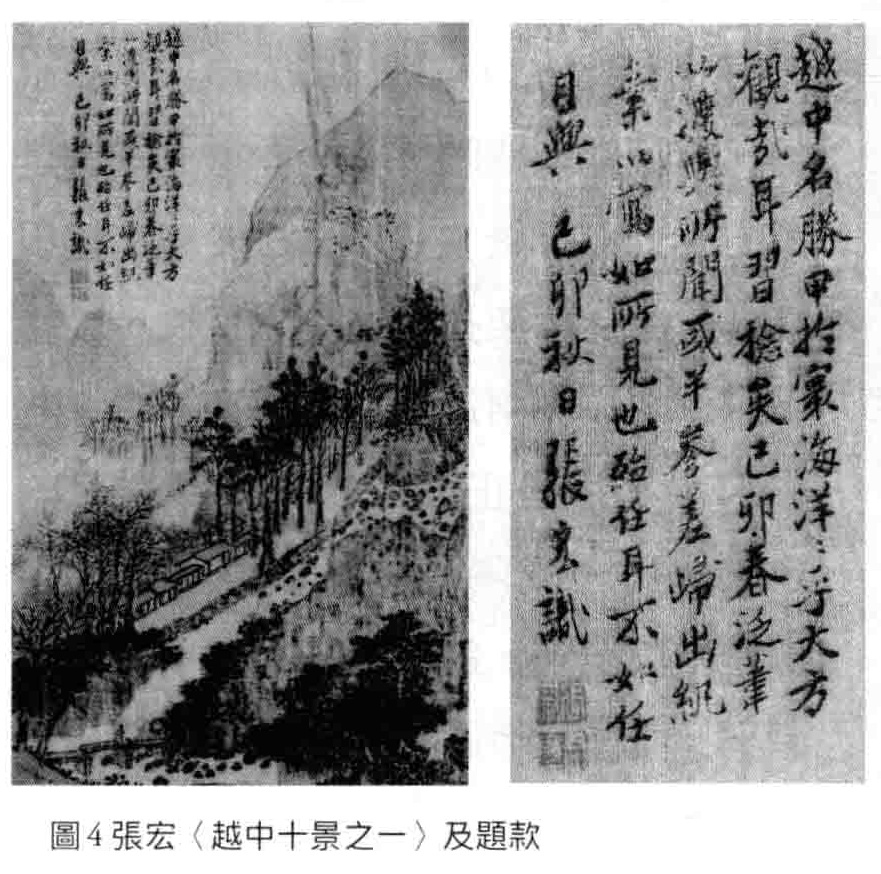
\includegraphics[width=\linewidth,height=.81\textheight,keepaspectratio]{assets/p018-01.jpg}
\end{minipage}
\hfill%
\begin{minipage}[t]{0.455\linewidth}
\vspace{0pt}\setlength{\parindent}{1.5em}
「笔法全无，虽工亦匠。」持的还是否定态度。古画论里多处提到画四时山川，有风雨明晦的观念。「明晦」何尝不是光线所致，我们也难得一见有所谓定向光影的画法。邹一桂这一记录的「皆有日影」，何以千年来的画家几乎都是「视而不见」？这是一个相当有趣的问题。〈长松图〉的画法是不是单纯的来自受西洋画法的启示？这又是一个有趣的问题。我想考虑西风东渐的反应，以当年的资讯流通状况，有

\end{minipage}
\par\addvspace{4pt}

\noindent 定向光影、单点透视的画风画家，都是看过西洋画吗？时代略早的张宏在〈越中十景之一〉（图4）（1639。奈良大和文华馆藏）题:「越中名胜，甲于寰海，洋洋乎大方观哉！耳习然矣。己卯春泛苇，以渡舆所闻，或半参差。归纳素以写，如所见也。殆任耳不如任目欤！己卯（1639）秋日张宏识。」好一句「任耳不如任目」，「任目」就是画眼中所见，忠实于自然，宋朝晁以道诗:「画写物外形，要物形不改。」当然看到光影画光影。往昔「任耳」，今以「以渡舆所闻」（任目）来印证所见，那前人所说（画），和眼中所见的实景，就是「或半参差。」我们也可以想到，中国人学画，大都是从临摹起步，不是面对真景，如今日所说的对景（物）「写生」，一旦养成习惯，古人怎么画，我就怎么画，古人不画「暗相」（阴

\vfill
\begin{BookNotes}
\BookNote{7.}{邹一桂《小山画谱》，收入《美术丛书》（五）初集第九辑，（台北：艺文，1975）页137-138。}
\end{BookNotes}

% 原图说　图4　张宏〈越中十景之一〉及题款

% 原书第 6 页（PDF 第 19 页）
\BookPage{6}{19}
\noindent 影），我就不画「暗相」。从张宏的其他作品，构图和当时流入中国的版画相当接近，研究者推论他受西洋的影响，有其图像上的证据。8那陆㬙呢？以今日所能得见的资料，恐难印证。对于有如本幅光影的表达，是来自画家的「任目」，或外来的因素，恐难说得清楚。

\par\addvspace{4pt}\noindent
\begin{minipage}[t]{0.532\linewidth}
\vspace{0pt}
\noindent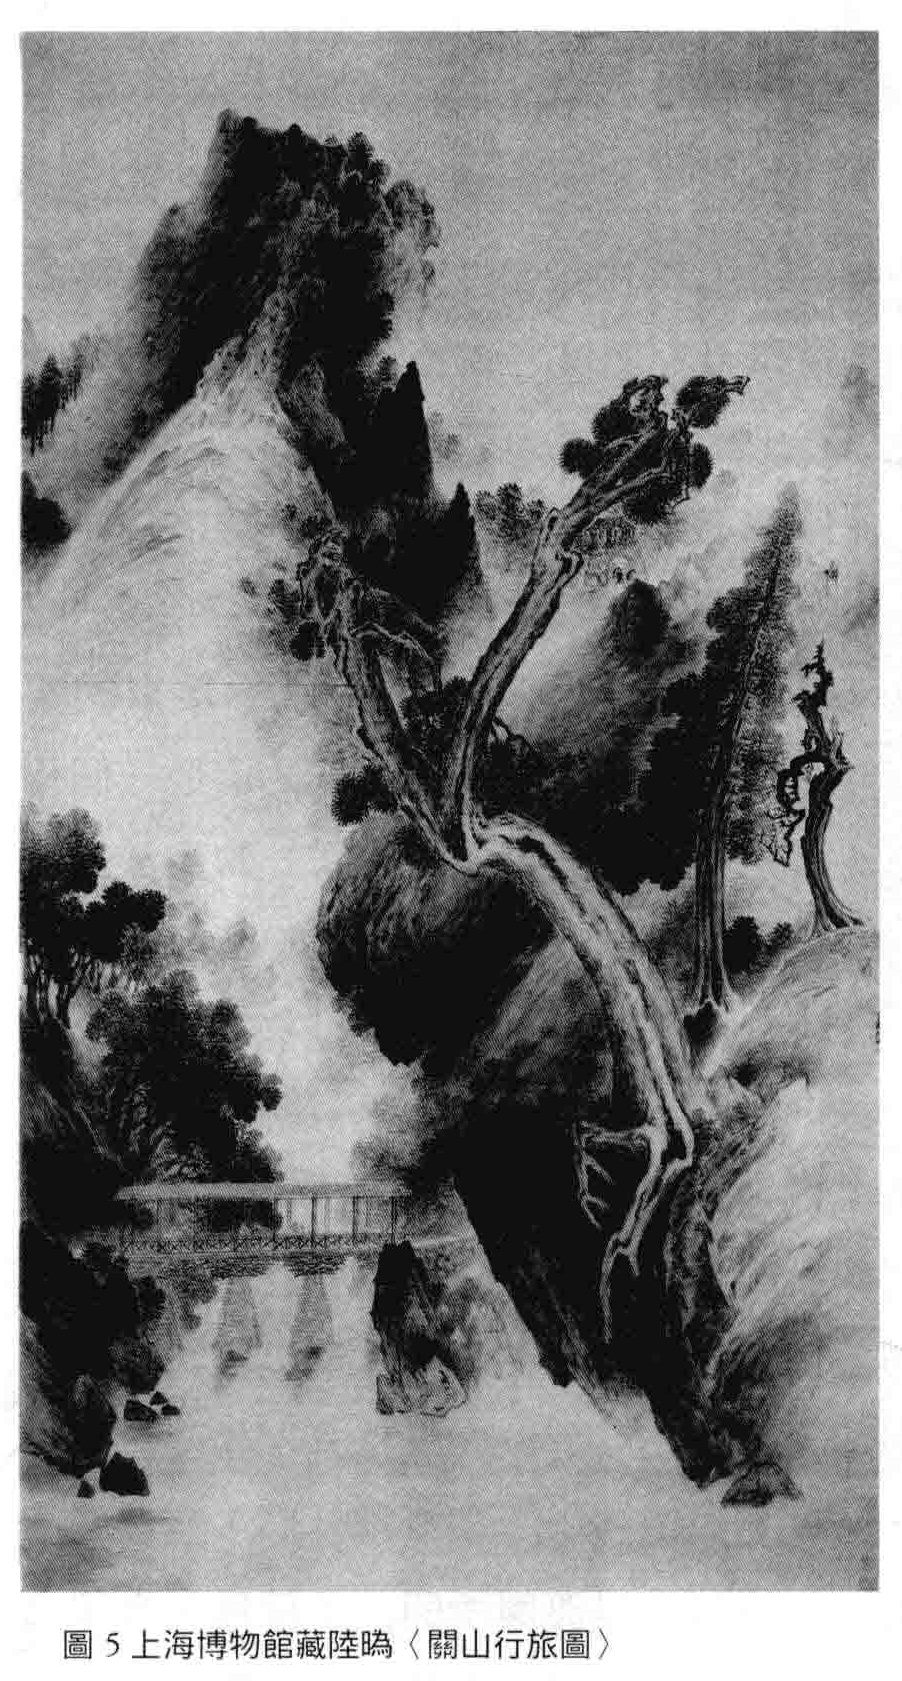
\includegraphics[width=\linewidth,height=.81\textheight,keepaspectratio]{assets/p019-01.jpg}
\end{minipage}
\hfill%
\begin{minipage}[t]{0.443\linewidth}
\vspace{0pt}\setlength{\parindent}{1.5em}
「任目」就能画出光影「暗相」的表达？上海博物馆藏陆㬙〈关山行旅图（图5，纵241.5公分，横129.6公分）。名为「关山行旅」，却置关隘于上方一小角，行旅进入关隘，骑座于道上，皆是远方小景。近景主要为长松于崖上盘根擎天，溪上横架长廊式遮阳平桥，松干下方，中亮，两边黑；高峰突起处，危崖临水，都是正面取光。主峰右旁的小尖山，不受阳光处，危崖下方，也都是施用浓墨。这是「暗相」。尤有甚者，〈关山行旅图〉平桥画出的桥墩，因水流所起的波动倒影，也都画出。此外，画幅右下角，也有倒影的出现。全幅看来，山川高下大小适宜，向背安放不失，大地的波光翠影，融于晨雾迷茫中。也就是光影与立体感的强调才能表达的。

\begin{BookQuote}
<长松图〉、〈关山行旅图〉，
\end{BookQuote}

画中松干的砢多节，盘根樛枝，皮

\end{minipage}
\par\addvspace{4pt}

\noindent 粗厚，松干明暗，用的是几近于中国画阴阳强烈对比。墨韵与笔触的融合，无中国人对西洋画「暗相」的突兀感。笔法犹是与中国无异的层层点画」，「具有醒人眼

\vfill
\begin{BookNotes}
\BookNote{8.}{高居翰着李佩华译《气势撼人》（台北：石头，1994)。本书的前部份，即以张宏为题论述。}
\end{BookNotes}

% 原图说　图5　上海博物馆藏陆㬙〈关山行旅图〉

% 原书第 7 页（PDF 第 20 页）
\BookPage{7}{20}
\noindent 目，虽工不匠，可入画品。

张庚《清朝画征录》谓「画宗二米、房山」，将陆㬙的画法归为「米氏云山」系统，指出墨韵的出处，但这是一种笼统的说法，何不说是「任耳不如任目」。上引《桐阴论画》:「一种奇古之气，与程穆倩相伯仲，境界灵异，别有会心，非巧思力索所能造也。」是对山川阳光的观察？或因缘际会于西风东渐的启示？何时才有正解。

\BookSubheading{(贰)}

<长松图〉只画松树，根如蹲虬，枝若交戟。枝干构成更有所指，画面上「影射」的是一个草书「寿」字的模样。兹以草书「寿」字并列来比较(图6）。草书「寿」字的写法，第一笔是上部的一横，接着是一竖而下，再过此「横划」转一个圈，左向斜出，再加一「横划」，上挑以后，再左斜下，又加一大横画，又左斜下反上转一圈，也有转两圈半者。〈长松图〉的上方及中幅斜向的松干，到最下坡上露根，就是对「寿」字的「影射」。从图版排列来对照，是相当清楚的。

松在古老的中国社会里与柏并举，认为是君子的象征，最为人熟悉的《论语》:「夏后氏以松，岁寒然后知松柏之后凋也。」松柏又成为「长寿」的一种比喻。晋左九嫔〈松柏赋〉曰:「何奇树之英蔚，…，赤松游其下而得道，文賔飡其实而长生，诗人歌其荣蔚，齐南山以永宁。」9道家的书籍，《玉策记》:「千岁松树，枝叶四边披起，上杪不长，望而视之，有如偃盖。其中有物，或如青牛，或如青犬，或如人，皆寿万岁。」1°《神仙传》:「松者横也，时受服者，皆至三百岁。」11《抱朴子》:「天陵偃盖之松，大谷倒生之柏，皆与天齐其长，地等其久。」12

实际以画松来作为祝寿，见唐代于邵（字相门，京兆万年人。天宝末，进士登

\vfill
\begin{BookNotes}
\BookNote{9.}{唐欧阳询撰《艺文类聚》(文渊阁四库全书本)卷八十八，页21。}
\BookNote{10.}{转引自《御定佩文斋广群芳谱》（文渊阁四库全书本)，卷六十八，页6。}
\BookNote{11.}{转引自《御定佩文斋广群芳谱》（文渊阁四库全书本），卷六十八，页6。}
\BookNote{12.}{转引自《御定佩文斋广群芳谱》（文渊阁四库全书本），卷六十八，页6。}
\end{BookNotes}

% 原书第 8 页（PDF 第 21 页）
\BookPage{8}{21}
\BookArt{p021-01.jpg}{0.990}{0.467}

\noindent 科）的文章，两次以画松献寿。〈吴使君厅郑华原壁画松树赞〉:「贵之者真，得之者难。松有劲质，匠乎笔端。森空倚，挺拔上干。如出绝壑，若生大寒。枝蟠龙变，皮折龟攒。青萝若挂，白鹭愁看。美华原之墨妙，能入室而思弹，愿主人之比寿，从君子之静观。」13唐德宗生日，于邵以〈进画松竹图表〉:「伏以今月十九日，累圣储休之日，陛下降诞之四月十九日生辰，…瞻北极而效诚，匝南山而献寿。…臣率鄙思，绘松竹图一面，并陈赞颂，…故臣绘长松，佐之修竹。…特最为有寿。…毫端敢借坚贞之姿，愿增天地之寿。」14

辽宁省博物馆宫藏明代朱瞻基（宣宗）所画〈万年松图卷〉（图7）。引首的自题楷书:「宣德六年四月初一日，长子皇帝瞻基敬写万年松图奉仁寿宫清玩。」画做于三十三岁，钤有「武英殿宝」，是为其母皇太后祝寿所作。

\vfill
\begin{BookNotes}
\BookNote{13.}{转引自《御定佩文斋广群芳谱》（文渊阁四库全书本），卷六十八，页28。}
\BookNote{14.}{宋李昉等编《文苑英华》，（文渊阁四库全书本），卷六百十三，页101。}
\end{BookNotes}

% 原图说　图6　草书「寿」字并列来比较（承吴嫦敏小姐制版，谨致谢意。）

% 原书第 9 页（PDF 第 22 页）
\BookPage{9}{22}
\BookArt{p022-01.jpg}{0.990}{0.429}

\par\addvspace{4pt}\noindent
\begin{minipage}[t]{0.460\linewidth}
\vspace{0pt}
\noindent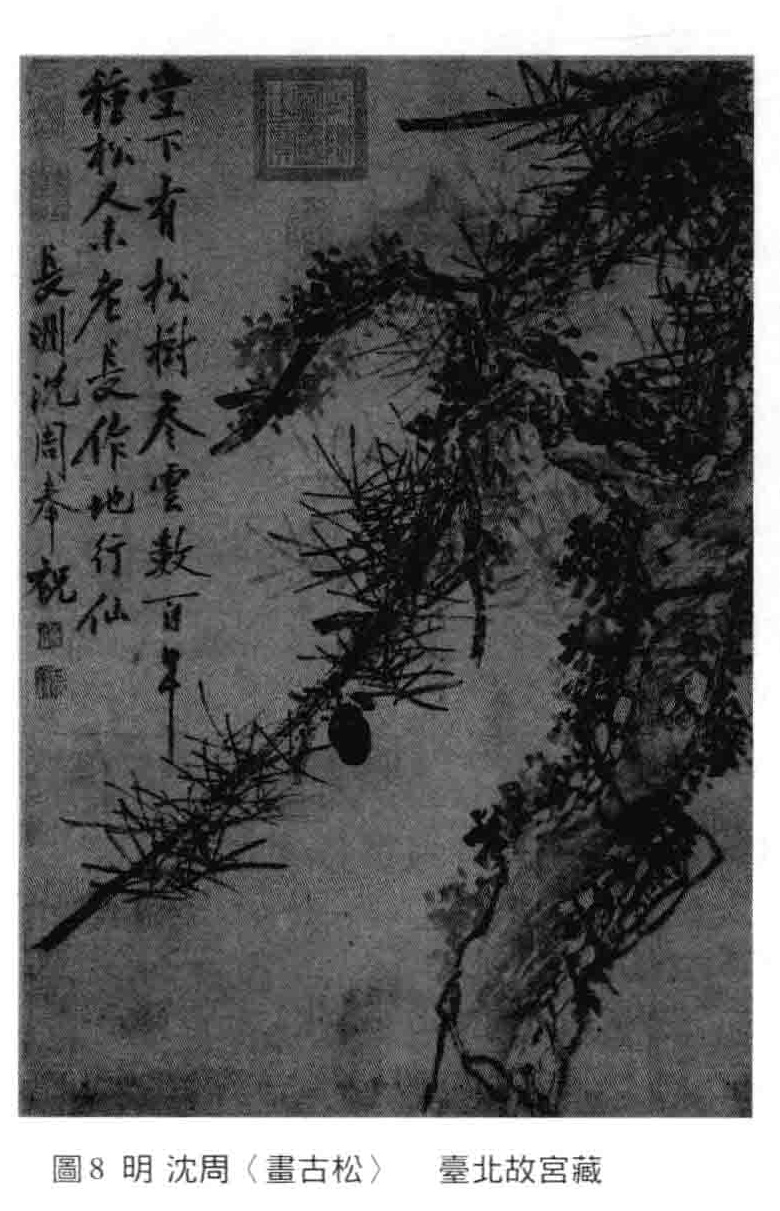
\includegraphics[width=\linewidth,height=.81\textheight,keepaspectratio]{assets/p022-02.jpg}
\end{minipage}
\hfill%
\begin{minipage}[t]{0.515\linewidth}
\vspace{0pt}\setlength{\parindent}{1.5em}
台北故宫藏明沈周有〈画古松〉（图8）。画上老松一株，藤萝盘缠，主干自左斜上，左方一枝几与主干相平行，用笔纵放而有力。款题:「堂下有松树，参云数百年。种松人未老，长作地行仙。长州沈周奉祝。」可知是为友祝寿所作。

以松柏画成「寿」字，陆㬙这〈长松图〉并非孤例。从乾隆的题画诗，见有两例。其一，〈题汪承霈画二幅〉：

湖石边旁古柏身，峙成寿字傍（(去声)长春（花名）。嘉其用意新非巧，小雅如歌天保人。（右古柏）横为岭也竖为峰，点画其间借老松。不似似中五福首。明几窗净伴清供。15（右山水)

\end{minipage}
\par\addvspace{4pt}

\vfill
\begin{BookNotes}
\BookNote{15.}{清弘历《御制诗集》（文渊阁四库全书本）卷三十九，页8。}
\end{BookNotes}

% 原图说　图7　朱瞻基（宣宗）所画〈万年松图卷〉局部一、二、三。　辽宁博物馆藏
% 原图说　图9　〈魁星踢斗〉

% 原图说　图8　明沈周〈画古松〉　台北故宫藏

% 原书第 10 页（PDF 第 23 页）
\BookPage{10}{23}
\noindent 其二，〈再题汪承霈画二幅〉：

\begin{BookQuote}
别裁巧不涉纤新，题句七旬忽八旬。(下小字注：戊申题承霈此画时年七旬有八，兹来重题，则已跻八旬。在承霈盖寓祝嘏之意，而予康强如昔，洵非易得。)漫向个中较六法，可知柏本寿为身。(右古柏）书中画复画中书，邱壑翻为寿字如。(下小字注：是幅山水布置，章法与古柏一幅，并成寿字。嘉其自出新意，即书即画，巧不涉纤，亦艺林中创见也。）试问千秋艺林者，独开生面孰同诸。（右山水）16
\end{BookQuote}

「书中画复画中书」，乾隆的用词相当精准。「不似似中五福首」，也就是指「寿」。「不似似中」也说明图与寿字之间，容许小有「考案」上的变化。可惜今日汪承霈的这两件尚在人间否？无从查知。陆㬙的〈长松图〉著录于《石渠宝笈》初编（乾隆十年完成），应该在汪承霈画作之前进宫。想来，乾隆的赞赏:「试问千秋艺林者，独开生面孰同诸。」忘了陆㬙的〈长松图〉所影射的「寿」字。

再说「书中画复画中书」，一个最佳的例子是「正心修身克己复礼」组成的<魁星踢斗〉（图9），至今犹普遍流行于民间。

\par\addvspace{4pt}\noindent
\begin{minipage}[t]{0.382\linewidth}
\vspace{0pt}
\noindent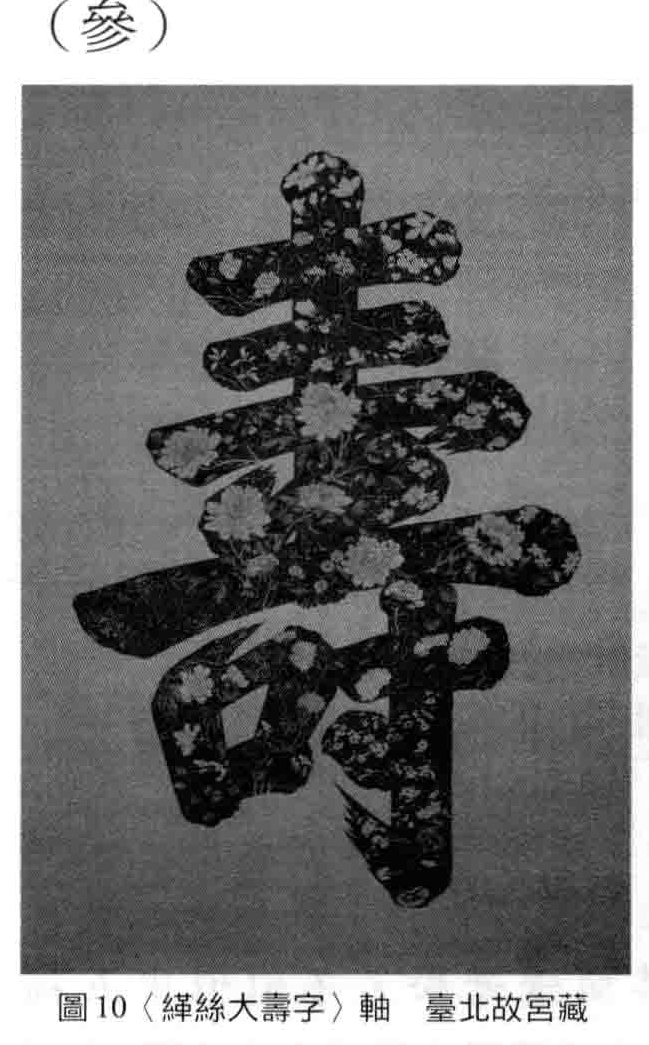
\includegraphics[width=\linewidth,height=.81\textheight,keepaspectratio]{assets/p023-01.jpg}
\end{minipage}
\hfill%
\begin{minipage}[t]{0.593\linewidth}
\vspace{0pt}\setlength{\parindent}{1.5em}
\noindent 〈縄丝大寿字〉轴。本幅纵208公分，横132.6公分；经62-66，纬96-128。刻织。白地朱色大寿字，笔划内刻以玉兰、牡丹、梅、玫瑰、紫藤、绣球花、水仙、海棠、灵芝诸花。(图10)

此幅织纹密匀，丝光犹新。众花仅刻织花瓣，枝干及叶之形状，再以色添染。各部细节为刻织兼画之作。图经朱启钤刻丝书画录著录，收传印记:清宣统玺。17

\end{minipage}
\par\addvspace{4pt}

\vfill
\begin{BookNotes}
\BookNote{16.}{清弘历《御制诗集》（文渊阁四库全书本)卷三十九，页7。}
\BookNote{17.}{图录见《国立故宫博物院缂丝.刺绣》（东京：株式会社学习，1970），（缂丝），五十七图。}
\end{BookNotes}

% 原图说　图10　〈缂丝大寿字〉轴　台北故宫藏

% 原书第 11 页（PDF 第 24 页）
\BookPage{11}{24}
<缂丝大寿字〉轴，本件未标示制作年代，从制作的技法，细节处为刻织兼画已是清代初年的制作法了。制作与同为台北故宫藏无名氏〈縄丝群仙祝寿〉（图11-1)是相同。〈缂丝群仙祝寿〉是典型的清院本纬丝。此幅坡石树干等处，皆为着笔塡染，略有郎世宁设色之阳光及当时画院繁缛琐碎之特色。再检视〈丝群仙祝寿〉与郎世宁的〈万寿同春〉（图11-2）比较，在画上所呈现的气息是相同的。〈万寿同春〉画中完全是中国传统青绿设色的岩石，这是出于画另一位宫廷画家唐岱之手，从唐岱的〈秋林读易〉（图11-3）岩石是同一手法得证。〈纬丝群仙祝寿〉原稿上的石也是唐岱所补。18以是可断定本件下限的年代为乾隆朝。

\BookArt{p024-01.jpg}{0.990}{0.418}

\vfill
\begin{BookNotes}
\BookNote{18.}{关于郎世宁画作中出现了纯中国笔法的合作画，常未具名是何画家合作。可见本人之著作，〈从故宫藏品探讨郎世宁的画风〉，收入天主教辅仁大学主编《郎世宁之艺术》（台北：幼狮，1991)，页21-43。又《内务府》（雍正七年流水档）记命唐岱与郎世宁合作画。「（八月）十七日，入画作，据圆明园来贴内称，本月十四日，郎中海望奉旨：九洲清宴『晏』东暖阁贴的玉堂春富贵横披画上玉兰花、石头甚不好，尔着郎石『世』宁画花卉，唐岱画石头。着伊二人商议画一张换上。钦此。」(3.640)}
\end{BookNotes}

% 原图说　图11-1　无名氏〈缂丝群仙祝寿〉台北故宫藏
% 原图说　图11-2　郎世宁的〈万寿同春〉台北故宫藏
% 原图说　图11-3　唐岱〈秋林读易〉台北故宫藏

% 原书第 12 页（PDF 第 25 页）
\BookPage{12}{25}
长寿是人生所憧憬的目标之一。人总是祈求长寿活得久为乐事。人生「五福」「寿」为先。19人生主观愿望的表示，传统的民俗生活里，中国传统吉祥纹饰，祝寿是一大宗。图样与文字，都是存在的。就长寿而言，用共识的象征，如本文的〈长松图〉以松献寿，乃至以鹤以龟（龟鹤齐龄）；以桃（蟠桃献寿。如麻姑献寿、东方朔偷桃；专用于女性的瑶池献寿）；用谐音格的「代代寿仙」（绶带鸟配寿石、桃花、水仙。）。「寿居耄耋」（寿石、菊『居』、猫、蝶。）。诸种象征义意义的传统吉祥纹饰，已具有长久的历史。

直接的以标出「寿」字为题，可见之于东汉代〈延年益寿大宜子孙锦〉（图12-1）（新疆考古学研究所藏）的织锦文，〈宋纬丝万寿图李咨颂〉（北京故宫藏）(图12-2）縄丝织出「寿」字；物件上如汉瓦当文的「延年益寿」（图12-3）、「千秋万岁」。

\BookArt{p025-01.jpg}{0.990}{0.448}

\vfill
\begin{BookNotes}
\BookNote{19.}{《尚书·洪范》：「五福，一曰寿，二曰福，三曰康宁，四曰攸好德，五曰考终命。」}
\end{BookNotes}

% 原图说　图12-1　东汉〈延年益寿大宜子孙锦〉新疆考古学研究所藏
% 原图说　图12-2　〈宋缂丝万寿图李诏颂〉台北故宫藏
% 原图说　图12-3　汉瓦当文的「延年益寿」
% 原图说　图13-1　民间工艺「团寿字」
% 原图说　图13-2　民间工艺「万寿」
% 原图说　图13-3　民间工艺方形化的「长寿字」

% 原书第 13 页（PDF 第 26 页）
\BookPage{13}{26}
「寿」之直接以文字表达，也非其他吉祥寓意的纹样所能比。「寿」这一文字从篆书到草、行、楷诸体，变化之多，尤其是篆字。篆书「寿」字的团形化，「团寿字」（图13-1）应用处最多，也许是是上下左右都对称，基本上文字已经图像化，所以应用于吉祥图案相当地方便。如再配以「卍」字，也是以左右对称设计，就是「万寿」(图13-2)；方形化的「长寿字」（图13-3）也是相同的意义。这种称为「寿字纹」，几乎把文字属性抽离，汉文字一字百写，也无他例了。所谓「百寿图」的出现，且流行至今。康熙六十岁（1713）寿庆，康熙五十六年（1717）武英殿版的《万寿盛典初集》，刊载了万寿盛典当日，由北京西郊畅春园至内城紫禁城神武门，一系列的祝寿活动。「直台路左为耆老接驾棚，前设龙亭御仗旗织，后张百寿黄幔长三丈，绣寿字百图。」20摆设龙亭，龙亭后有百寿黄幔并绣〈寿字百图>(图14)。

至于寿字和图画配合，「寿」字配五只蝙蝠为〈五福拜寿（图15-1）；长春花配「万寿」（图15-2）两字。「福鹿同寿」（图15-3）等等，不胜枚举，这都是民俗生活中所常见的。

\BookArt{p026-01.jpg}{0.990}{0.358}

\vfill
\begin{BookNotes}
\BookNote{20.}{《万寿盛典初集》（文渊阁四库全书本），卷四十三，页6。}
\end{BookNotes}

% 原图说　图14　武英殿版《万寿盛典初集》百寿黄幔并绣〈寿字百图〉台北故宫藏
% 原图说　图15-1　民间工艺〈五福拜寿〉

% 原书第 14 页（PDF 第 27 页）
\BookPage{14}{27}
\BookArt{p027-01.jpg}{0.988}{0.258}

\par\addvspace{4pt}\noindent
\begin{minipage}[t]{0.472\linewidth}
\vspace{0pt}
\noindent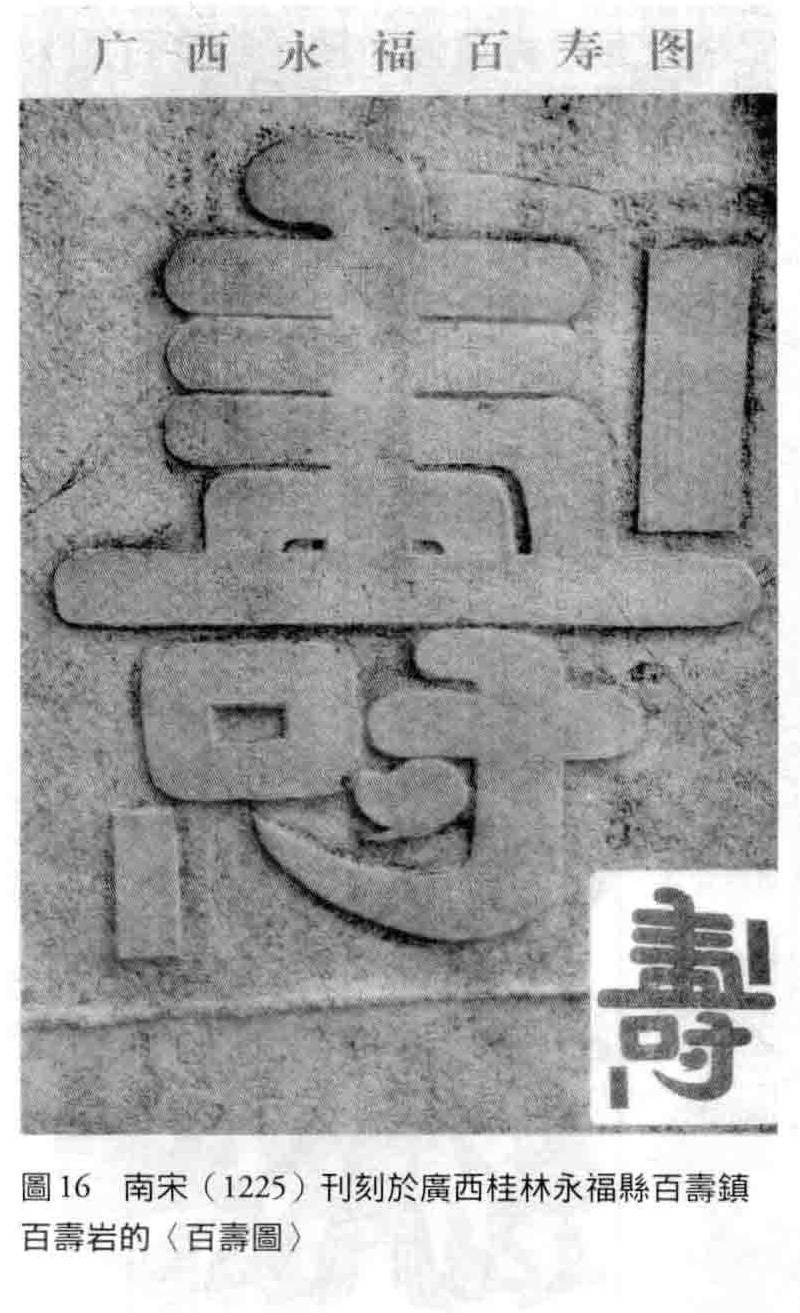
\includegraphics[width=\linewidth,height=.81\textheight,keepaspectratio]{assets/p027-02.jpg}
\end{minipage}
\hfill%
\begin{minipage}[t]{0.503\linewidth}
\vspace{0pt}\setlength{\parindent}{1.5em}
\begin{BookQuote}
〈纬丝大寿字〉轴直接以楷书一大寿
\end{BookQuote}

字来祝福。存世「大寿字」，得见于南宋(1225）刊刻于广西桂林永福县百寿镇百寿岩的〈百寿图〉（纵175公分，横148公分）（图16）字是隶书近楷，且在大寿字笔划中，刻有一百个小寿字。21

\begin{BookQuote}
〈丝大寿字〉轴，以「颜体赵面」的
\end{BookQuote}

「馆阁体」楷书书法写出。织品的字迹字大几近一百五十公分高，「大字难于结密而无间」，这是因为字大恐流于空疏，支撑不住大书幅。本幅寿字的结体，笔顺的点划起落转折，笔划之间的「布白」，都是中规中矩毫无失准，且显出一股庄重雍容，富厚雄健的气息。整幅以近朱红为笔划，粉朱花朵配绿叶，锦光为底，色彩的搭配。喜艳抢眼，无庶民之俗，而是皇家贵气。清皇帝制作的

\end{minipage}
\par\addvspace{4pt}

\noindent 记录，有一例，见于康熙皇帝〈恭祝皇太后万寿无疆赋〉:「织寿字以成图；捧霞

\vfill
\begin{BookNotes}
\BookNote{21.}{见邱明波，〈广西永福百寿图意象分析〉《南方文物》2010.2。所附图版。又见，（清）姚启瑞纂修；李文凡，李晨生点注；马夏民审校：《永宁州志》，山西古籍出版社，1996年。}
\end{BookNotes}

% 原图说　图15-2　民间工艺长春花配「万寿」
% 原图说　图15-3　民间工艺福鹿同寿

% 原图说　图16　南宋（1225）刊刻于广西桂林永福县百寿镇百寿岩的〈百寿图〉

% 原书第 15 页（PDF 第 28 页）
\BookPage{15}{28}
\noindent 觞而进。」22简易的书写「寿」字以应景。乾隆〈元旦试笔〉诗:「慈宁曙色霭昕昕，贺祚躬携百辟寿。母望九年子望七，今稀遇事古稀闻。椒花自献祥图颂，鼎篆旋成『寿』字文。屈指元正经四度，重循庆典倍虔欣。六街响卜是宫音…。」23这是乾隆元旦时为母庆寿也为自己祝寿，书写了「寿」字。另外，对于臣下的赐礼，书写「寿」字，现存于山东曲阜孔府，有道光二十二年赏赐衍圣公孔繁灏的〈福寿〉（碑）（图17-1）；光绪二十二年慈禧太后御笔赏赐孔令贻诰封一品夫人的〈寿）字（碑)（图17-2）。到了蒋中正总统主政，尚有此书写大寿字为贺的习惯（图17-3）。现代工艺的「寿」字，也见到民间使用（图17-4）。

\BookArt{p028-01.jpg}{0.990}{0.384}

\begin{BookQuote}
〈绎丝大寿字〉配上「玉兰、牡丹、梅、玫瑰、紫藤、绣球花、水仙、海棠、
\end{BookQuote}

灵芝」诸花。寓意上，借助天地万物之力，以植物象征，求长寿之欢乐，一如群卉来祝，蓬勃的繁花锦簇，挂上墙，满堂喜气洋洋。这种「造意」的添加，如今日尚存的工艺品，如前举现代工艺的「寿」字，加上神仙人物，也是一例（图17-4）。从美术的关点，这也就是汉字的装饰艺术。汉字造字，「象形」是其一，以形示意，以

\vfill
\begin{BookNotes}
\BookNote{22.}{清玄烨（圣祖）《御制文》（文渊阁四库全书本），第2集，卷四十二，「赋」，页1。}
\BookNote{23.}{清弘历（乾隆）《御制诗集》〈元旦试笔〉诗（文渊阁四库全书本）卷四十一，页1。}
\end{BookNotes}

% 原图说　图17-1　道光二十二年赏赐衍圣公孔繁灏〈福寿〉（碑）
% 原图说　图17-2　光绪二十二年慈禧太后御笔赏赐孔令贻诰封一品夫人〈寿〉字（碑）
% 原图说　图17-3　蒋中正总统书写「寿」字　小中堂
% 原图说　图17-4　现代工艺「寿」字加上神仙

% 原书第 16 页（PDF 第 29 页）
\BookPage{16}{29}
\noindent 意传情，进而将之图像化，用以满足视觉心理的要求，应用于审美活动，也是顺理成章。汉字字体的装饰艺术相当长远，如春秋时期的鸟虫篆（殳书）即是，往后，将字体装饰美化、图案化，历朝相当丰富。吉祥纹饰中所使用的文字，可说已演变成专门的工艺艺术了。

发掘文字的各种可能性，并利用文字造型的灵活性，来和图像与生活经验相结合。〈长松图〉、〈縄丝大寿字〉把松、花卉融入字体之中，更能满足吉祥的愿望。这不关贵族庶民，生活上都做如是观。
